\section{Exploratory Data Analysis}

\begin{frame}
  Exploratory Data Analysis
\end{frame}

\begin{frame}
  \frametitle{Brazilian fire foci aggregated by month (all years)}
    \begin{figure}
      \centering
      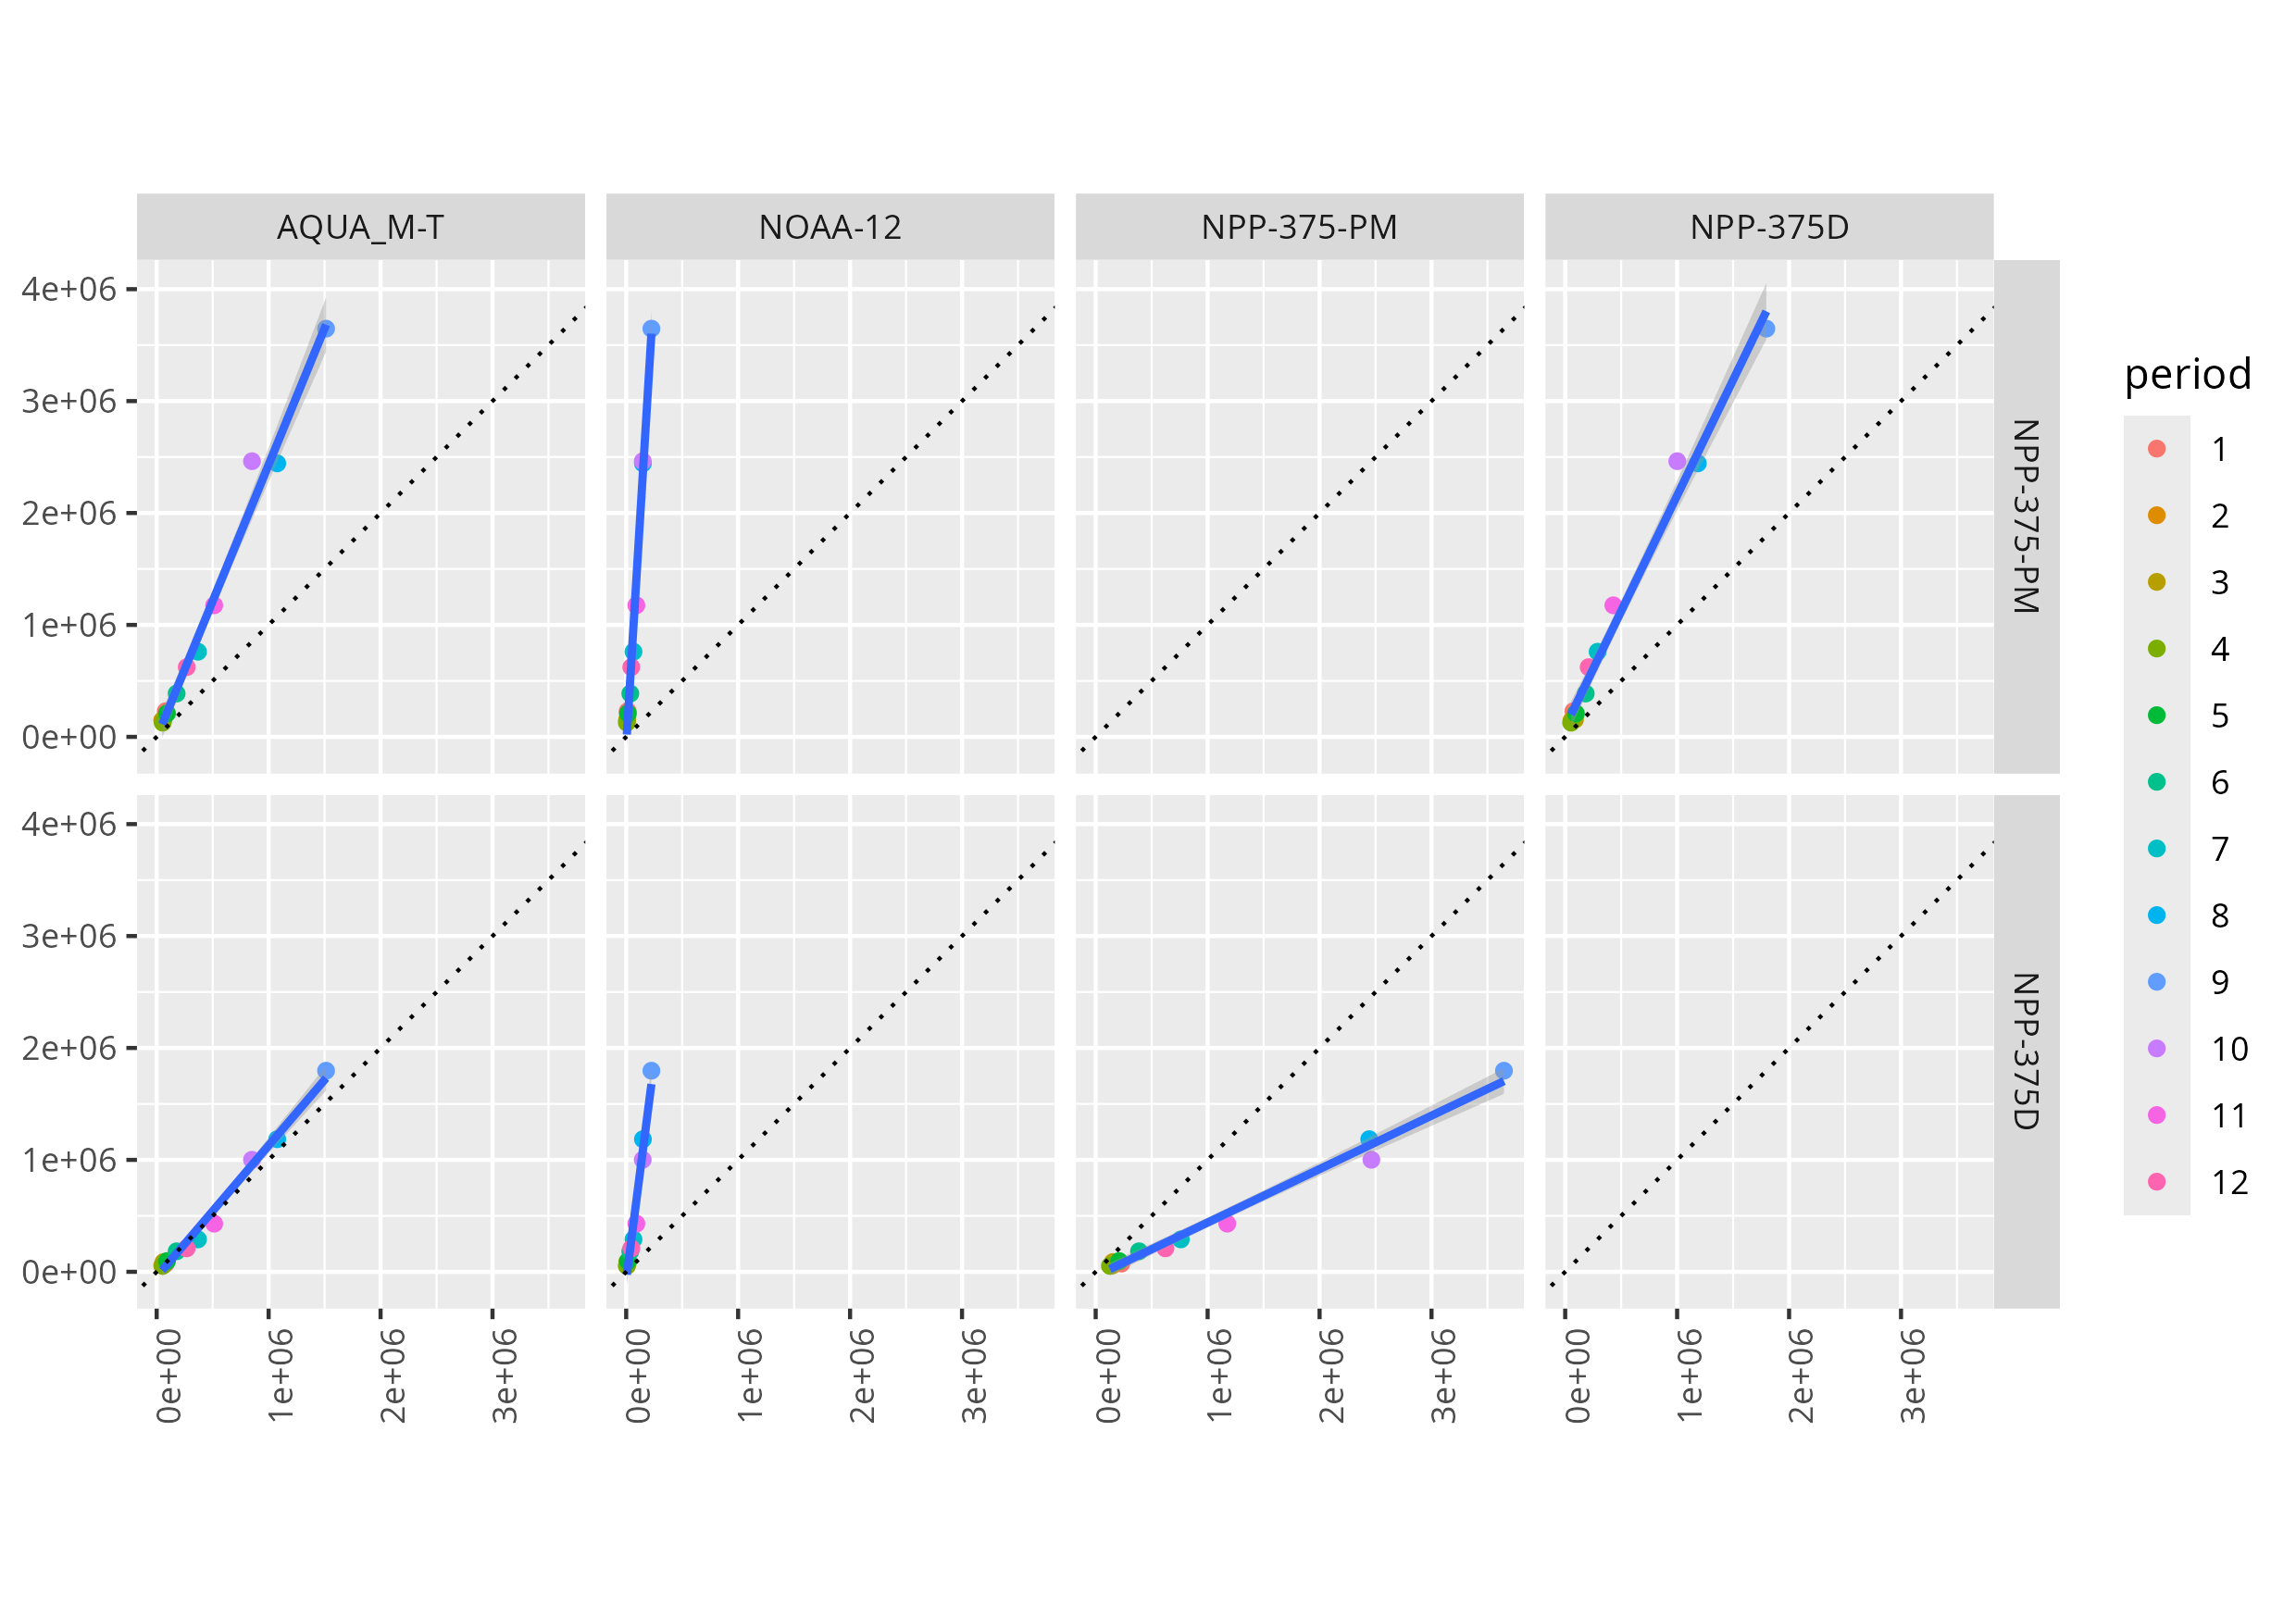
\includegraphics[scale=0.5]{figures/plot_lm_brazil_month.png}
    \end{figure}
\end{frame}

\begin{frame}
  \frametitle{Brazilian fire foci aggregated by year and month}
    \begin{figure}
      \centering
      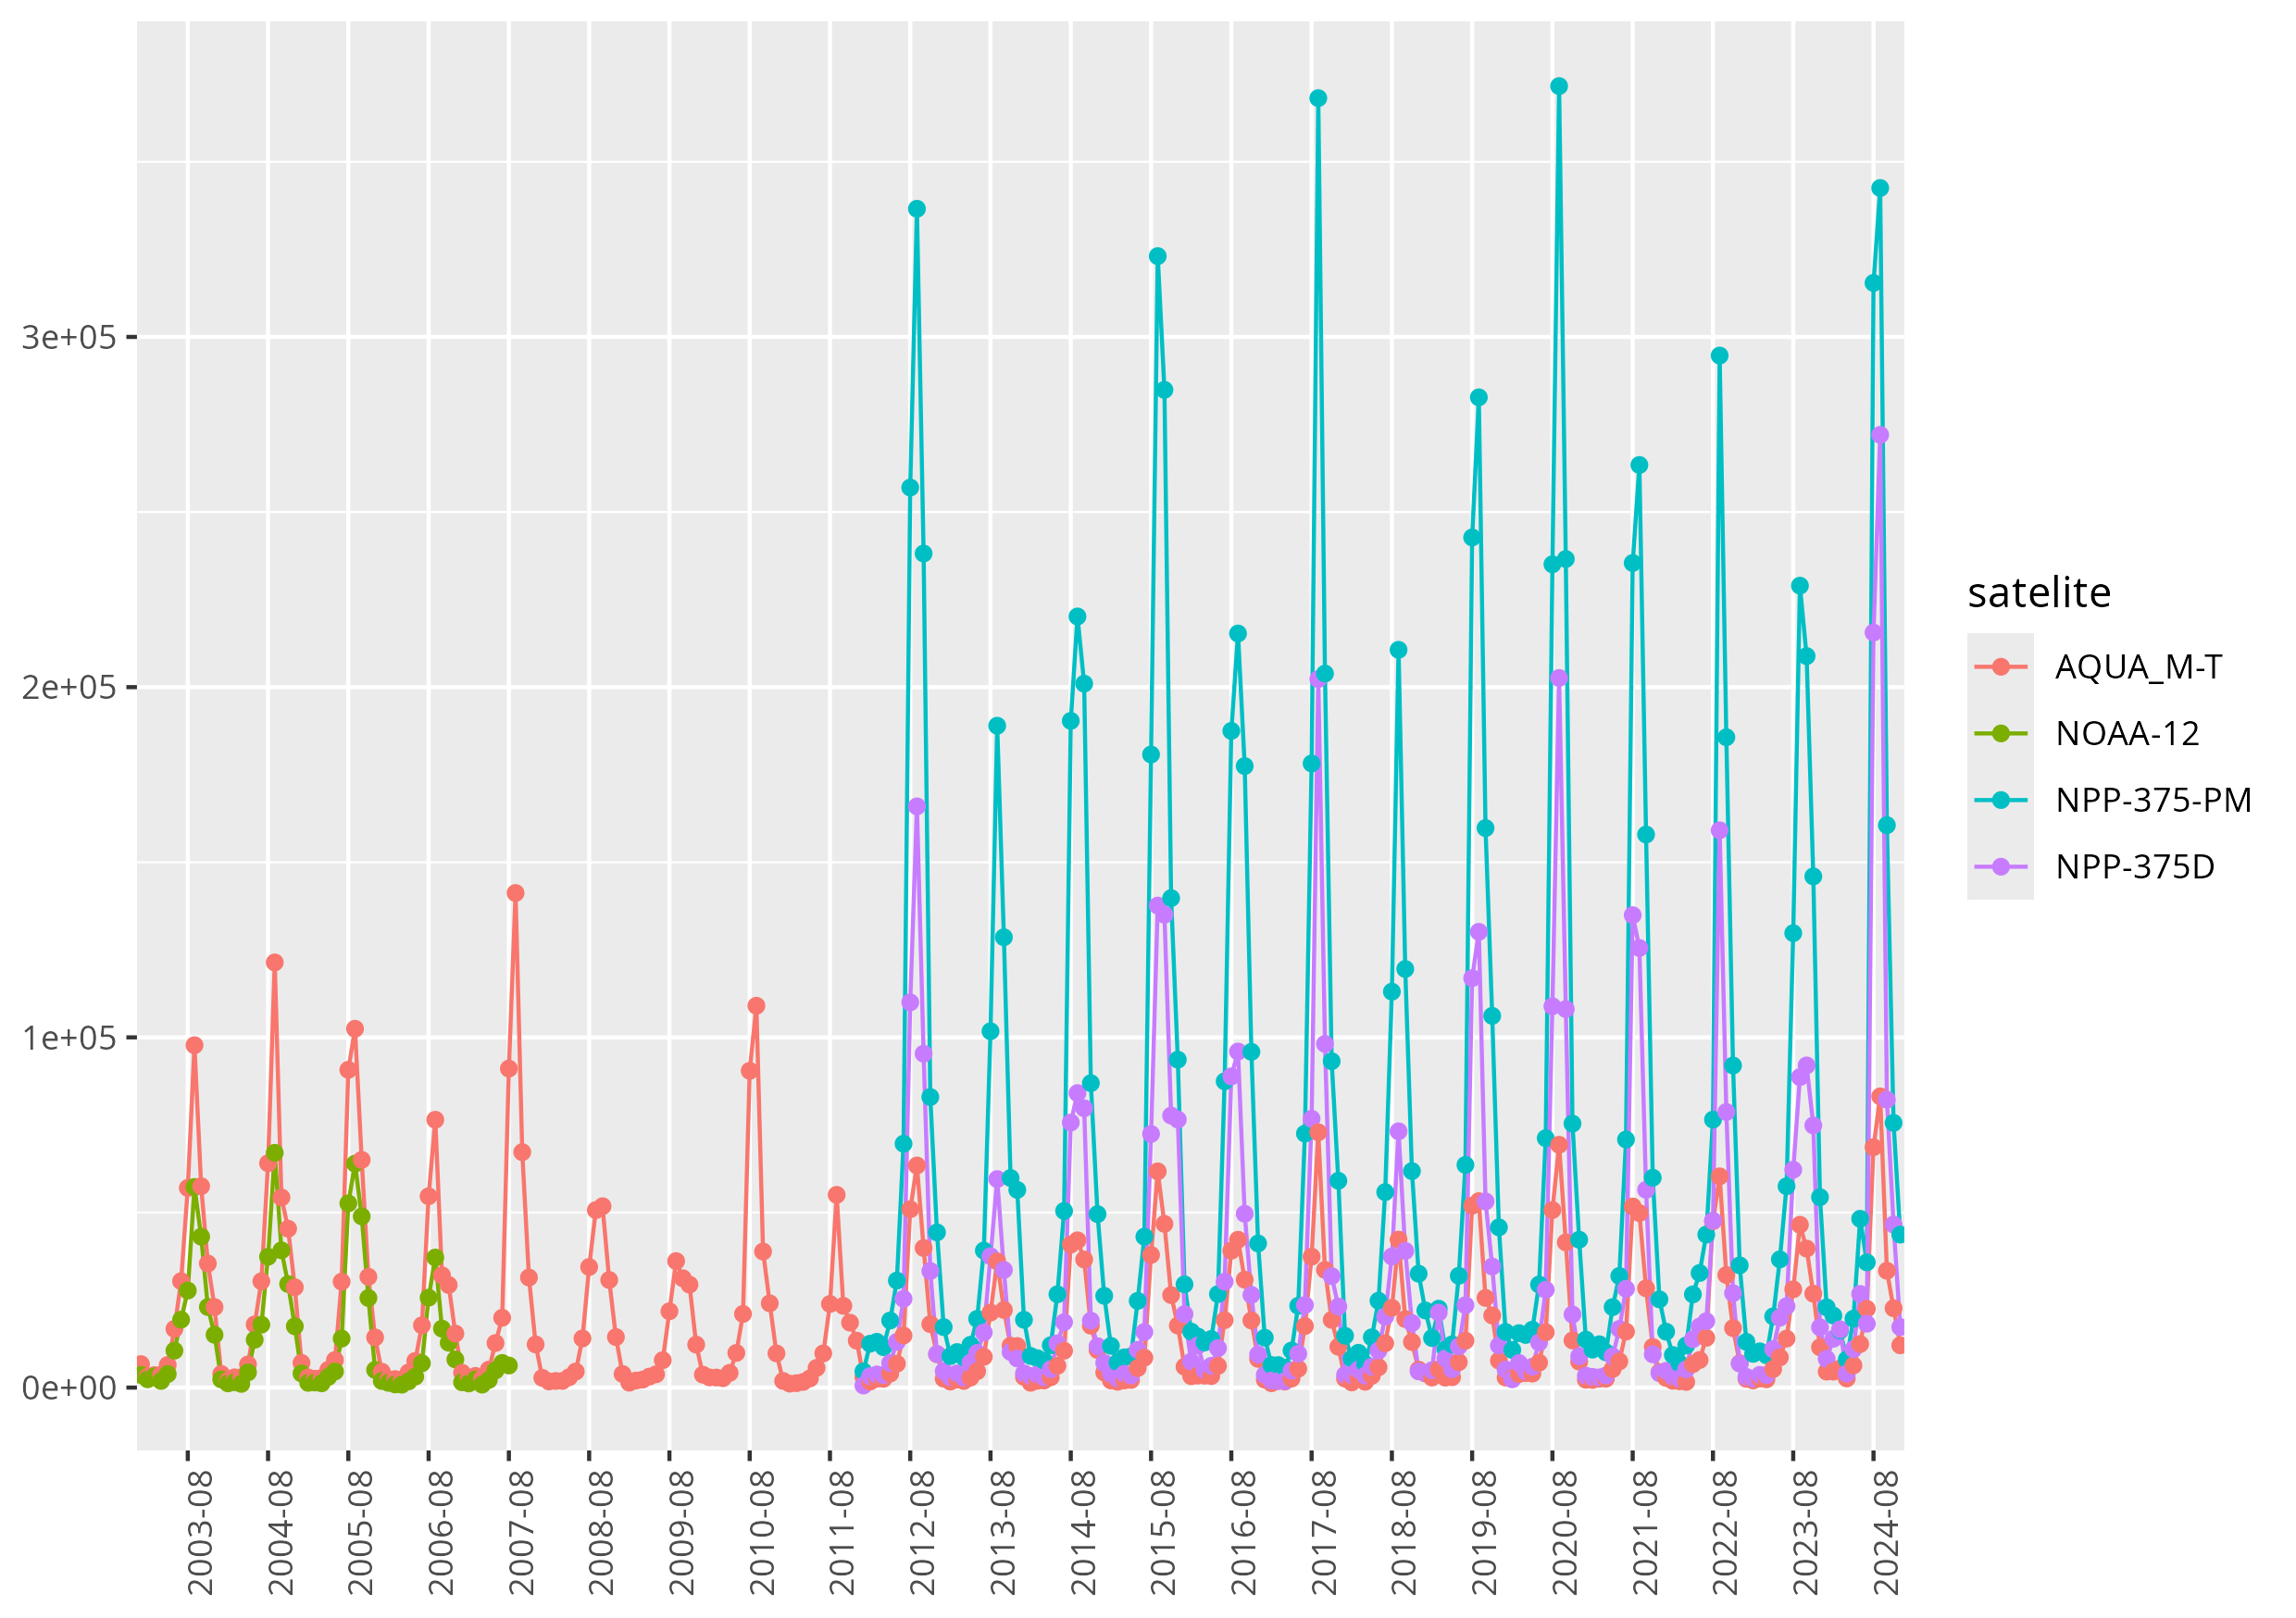
\includegraphics[scale=0.5]{figures/plot_line_brazil_year_month.png}
    \end{figure}
\end{frame}

\begin{frame}
  \frametitle{Correlation between fire foci from the reference satellites in Brazil}
  \begin{columns}
    \begin{column}{0.5\textwidth}
      \begin{itemize}
        \item The time series overlap partially.
        \item Use only the month (not the year) to compute correlation.
        \item This way we can use the whole time series in the estimation.
      \end{itemize}
    \end{column}
    \begin{column}{0.5\textwidth}
    \begin{figure}
      \centering
      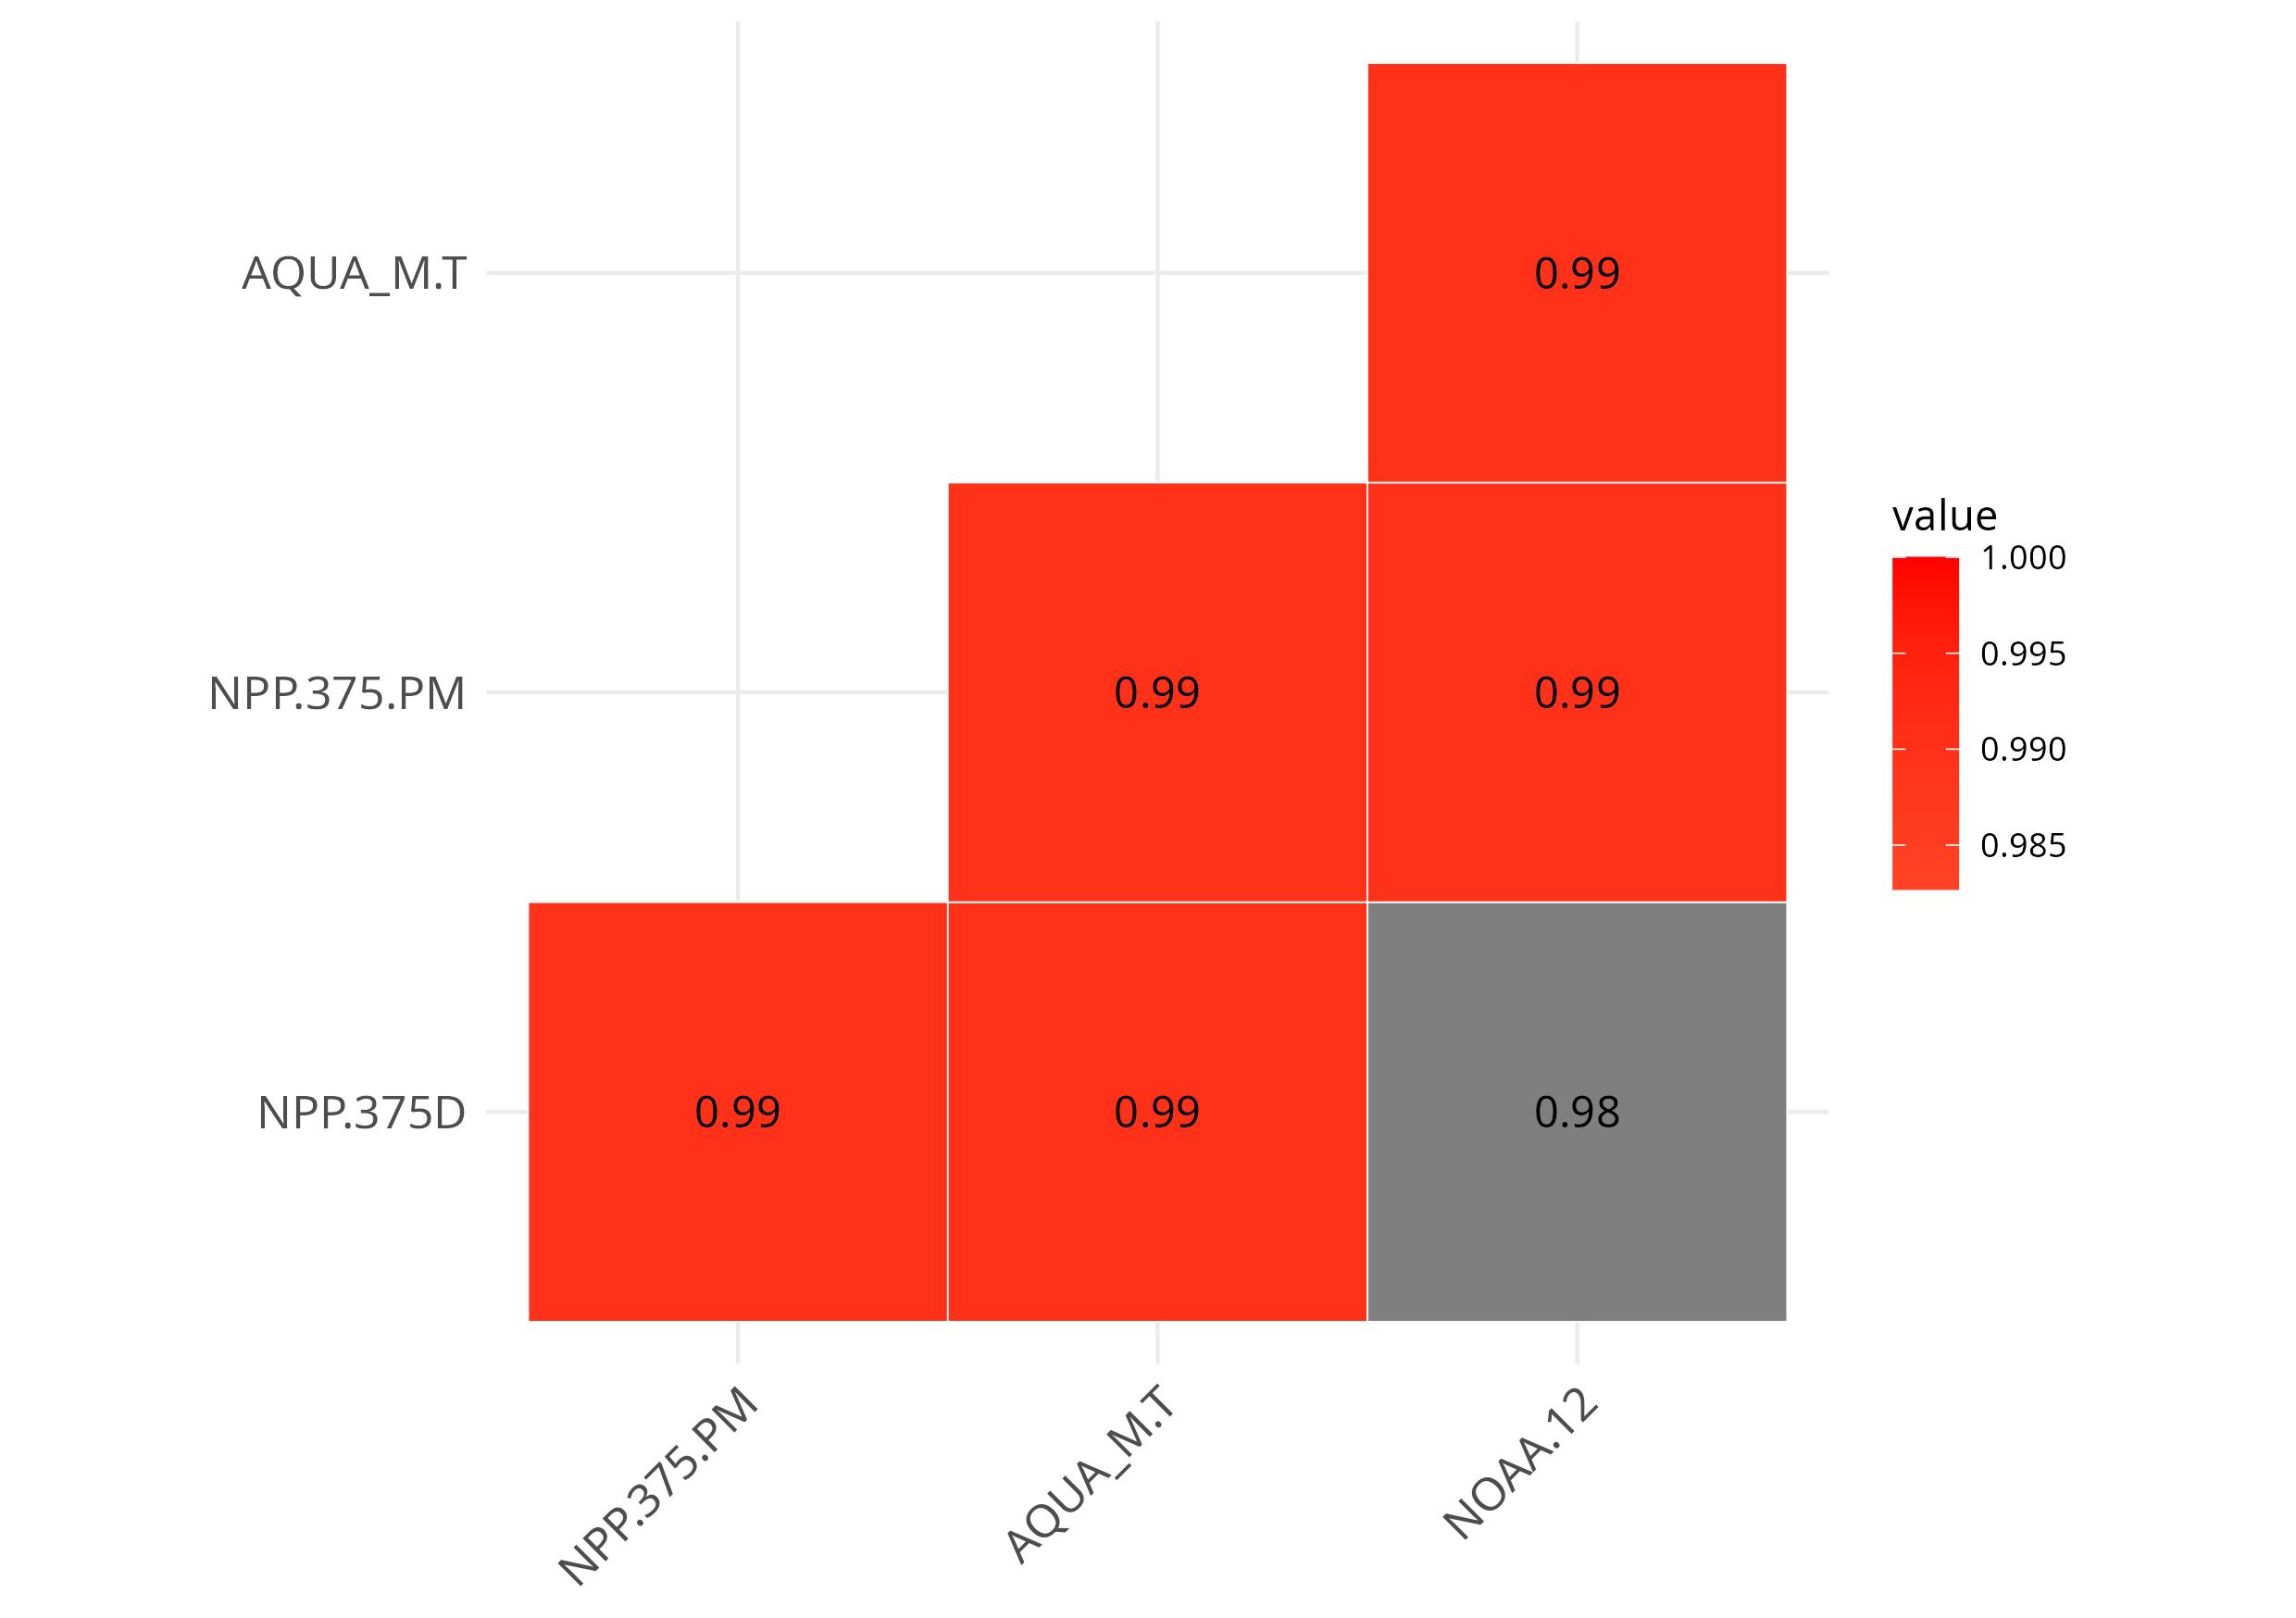
\includegraphics[scale=0.37]{figures/plot_cor_brazil_month.png}
    \end{figure}
  \end{column}
  \end{columns}
\end{frame}

\begin{frame}
  \frametitle{Correlation between fire foci from the reference satellites in Brazil}
  \begin{columns}
    \begin{column}{0.5\textwidth}
      \begin{itemize}
        \item The time series overlap partially.
        \item Estimate the correlation using only observation that overlap.
        \item Some satellites don't overlap and their correlation can't be
          estimated.
      \end{itemize}
    \end{column}
    \begin{column}{0.5\textwidth}
  \centering
  \csvautotabular{tables/correlation_overlapping_ts.csv}
    \end{column}
  \end{columns}
\end{frame}

\begin{frame}
  \frametitle{Brazilian regions by year and month}
    \begin{figure}
      \centering
      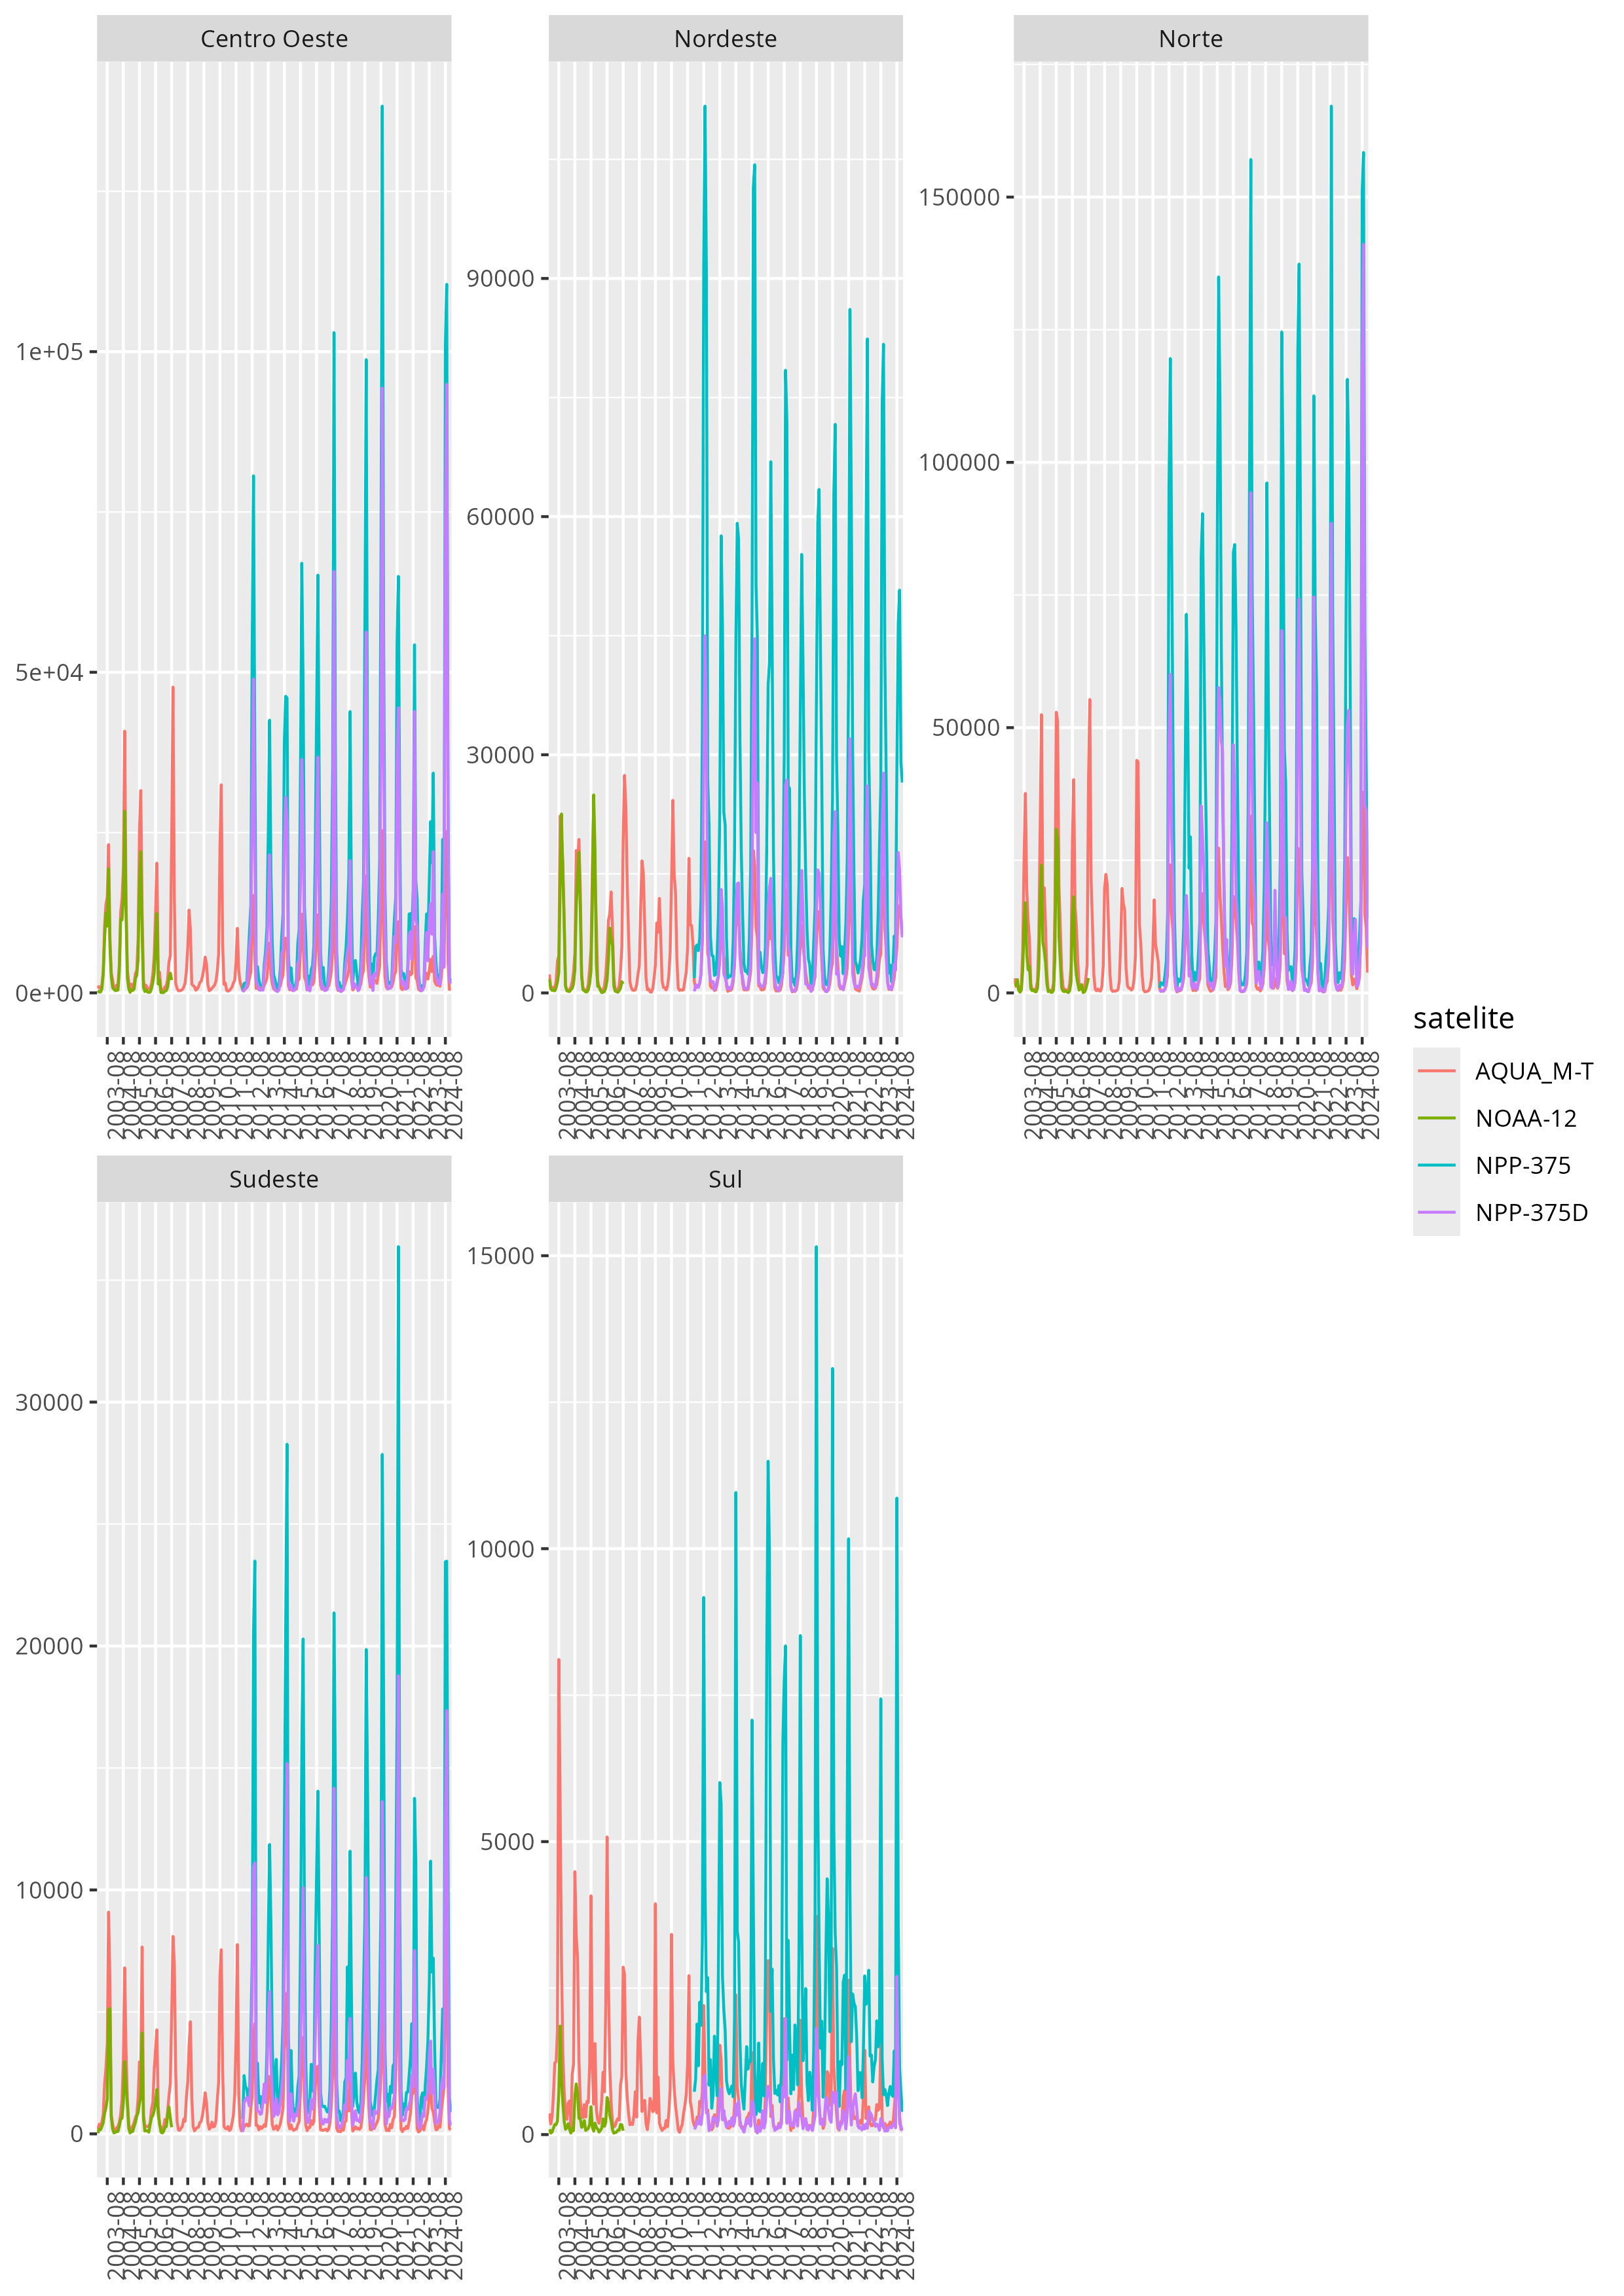
\includegraphics[scale=0.35]{figures/plot_line_brazil_region_year_month.png}
    \end{figure}
\end{frame}
